%\documentclass[review]{elsarticle}
\documentclass[twocolumn,5p,12pt]{elsarticle}
%%%%%%%%%%%%%%%%%%%%%%%%%%%%%%%%%%%%%%%%%%%%%%%%%%%%%%%%%%%%%%%%%%%%%%%%%%%%%%%%%%%%%%%%%%%%%%%%%%%%%%%%%%%%%%%%%%%%%%%%%%%%
\usepackage{lineno,hyperref}
\modulolinenumbers[5]
\journal{Physica A}
\bibliographystyle{elsarticle-num}
%%%%%%%%%%%%%%%%%%%%%%%

\usepackage{graphicx} % Include figure files
\usepackage{dcolumn}  % Align table columns on decimal point
\usepackage{bm}       % bold math
\usepackage{amsmath}
%\usepackage{amsfonts}
\usepackage{amssymb}
\usepackage[english]{babel}

\author[1]{J.B. Santos-Filho\corref{mycorrespondingauthor}}
\cortext[mycorrespondingauthor]{Corresponding author}
\ead{joao.batista@ifs.edu.br}
\author[1]{J.A. Plaskac}
\author[2]{T.S. de Araujo Batista}
\author[1]{}
\author[1]{}
\address[1]{}
\address[2]{}

\begin{document}

\begin{frontmatter}

\title{Aluminum cluster in the Fe-Al alloy to explain the anomalous behavior of the phase transition diagram.}


\begin{abstract}
%
%
\end{abstract}

\begin{keyword}
site-diluted Ising model\sep
Fe-Al alloys  \sep
Monte Carlo simulations \sep
phase transition diagram
\end{keyword}
\end{frontmatter}

%\linenumbers
%\pacs{:}
%\maketitle

\section{Introduction}

The magnetic and structural properties of Iron aluminides has been widely studied during many years\cite{Domb1983, Kubaschewski1982}, due its exhibit industrial applications properties such as oxidation and corrosion resistance, good ductility at room temperature, relatively low density, high magnetic permeability value, good vibration damping and insulation properties. Recent studies also have shown that alloys Fe-Al are promising candidates for data storage with magnetic patterns at room temperature \cite{Menendez2009,Bali2014}.  On the other hand, the magnetic properties of Fe-Al alloys are strongly linked with their chemical structure, the alloy can behave as ferromagnetic or paramagnetic at room temperature   depending of composition and synthesis method \cite{Wolf11986,Besnus1975,Dias2009,Oubelkacem2010}. It is also possible to induce new types of critical behavior as superparamagnetism and reentrant spin glass phase \cite{Arrott1959,Shull1959,Boni1986,Takahashi1996}. These characteristics have made this alloy one of the most studied binary systems in both experimental and theoretical research points of view.

	The disordered Fe-Al alloys are arranged on body centered cubic (bcc)  lattice structure, which may be represented by Fe$_{1-p}$Al$_{p}$, where $p$ is the concentration of aluminum. In the range of $0 <p <0.18$ the alloy is in a disordered ferromagnetic phase known as phase $A2$ \cite{Sort2006,Trautvetter2011,Zamora2009}, it is structurally disordered independent of the heat treatment \cite{Kubaschewski1982}. In this interval there is a small variation of the critical temperature as a function of the concentration q, and the temperatulanguage-latexre only decreases to $p> 0.1$ in contrast to the theoretical predictions, where for finite systems a finite inclination of the transition temperature at $q = 0$ \cite{Domb1983}. For $p> 0.18$ obtaining the alloy in the disordered phase depends on the synthesis process. For $0.2<  p <0.3$ the diagram shows a steep slope and vanishes in  $p = 0.7$.

	In order to try explain this anomalous behavior of phase transition diagram we propose an extended version of the site-diluted Ising model, following the same lines as the previous works on Fe-Al whose interaction of ferromagnetic exchange between Fe-Fe decreases linearly with the increase of $p$ \cite{x,x1,Plascak2000}. This is due to the expansion that is produced when Al atoms replace Fe atoms in a BCC network as a consequence of their larger atomic size. Also we consider in the model that Al atoms on small clusters can induce an extra super-exchange like ferromagnetic interaction between second-neighbors Fe atoms. Similar to the model used by Plascak and co-workers \cite{Plascak2000}, differentiating only that the superexchange is constant and is not induced by Al atoms on large clusters.

	We know from the advent of nanotechnology that the elements behave very differently when their dimensions are reduced to the point of being formed by a "countable" number of atoms \cite{Koch2006}. Recently researchers have shown for example that the cluster of $102$ gold atoms behaves as a giant molecule and not as metal. While clusters with $144$ atoms exhibit a metallic behavior \cite{Mustalahti2015}. By analogy, this behavior depending only on the number of atoms in the cluster can be used to obtain the behavior of the phase diagram of the alloy of Fe-Al. For this we must visualize the system as being composed of different aluminum clusters dispersed in an iron lattice. In the proposed model we consider that some clusters of aluminum contribute to induce a superexchange interaction and others do not, depending of the clusters size.

 	In this work we report the calculated critical temperature e magnetics proprieties site bond diluted Ising model with superexchange interaction on BBC lattice. While the Ising model is not completely appropriate for the study of these alloys,there is some experimental evidence reinforcing the choice of such localized models instead of the itinerant ones, mainly due the constant average Fe magnetic moment  as discoursed in Ref. \cite{Perez1986}.

\section{Model and calculations}
The system under investigation is given by a quenched site-diluted Ising model, Hamiltonian defined on a Body Centered Cubic lattice with $N$ sites, that can be
\begin{eqnarray}\label{hamil}
\begin{split}
\mathcal{H} =-J_1(p)&\sum_{\langle NN\rangle} \epsilon_i \epsilon_jS_{i}S_{j} \\& ~- J_{2}\sum_{\langle NNN \rangle}\zeta_{ij}  \epsilon_i \epsilon_j S_{i}S_{j}
~,
\end{split}
\end{eqnarray}
%
where the first sum is over nearest-neighbors ($NN$) pair and the second sum over next-nearest-neighbors ($NNN$) pairs, $S_i$ represents a $1/2$ Ising spin. $J_1(p)=J(1- \alpha p)$ is the first-neighbor interaction, it’s a linear function of contraction $p$, and $J_2=\beta J$ is the second-neighbor interaction, it’s a constant ferromagnetic interactions. In Eq.(\ref{hamil}), $\epsilon_i$ are quenched, uncorrelated random variables, representing the existence of two kinds of particles in the system, namely the magnetic ones with $\epsilon_i=1$, and non-magnetic ones with $\epsilon_i=0$. The variable $\epsilon_i$ is chosen according to the probability distribution
%
\begin{equation}
P(\epsilon_i) = p\delta(\epsilon_i-1) + (1-p)\delta(\epsilon_i),
\label{pro}
\end{equation}
%
where $p$ is the concentration of no-magnetic sites, such that $p = 0$ corresponds to the pure case. In Eq.(\ref{hamil}),  $\zeta_{ij}=1$ or $0$ whether or not there is superexchange interaction. There are an Superexchange interaction between the next-nearest-neighbor pairs when an aluminum atom is present as $NN$, and if this atom is on a cluster with lesss equal of $\Gamma$ aluminum atoms. In a quenched dilution, the increase in concentration $p$ leads to the formation of Al clusters. Since the probability of finding a cluster with $\Gamma$ Al atoms depends of $p$, the parameter $\Gamma$ indirectly connects $J_2$ to the concentration $p$.

\begin{figure}[!t]
  \centering
   \hspace{0.8cm}
 {\scriptsize\textbf{(a)}}\\
   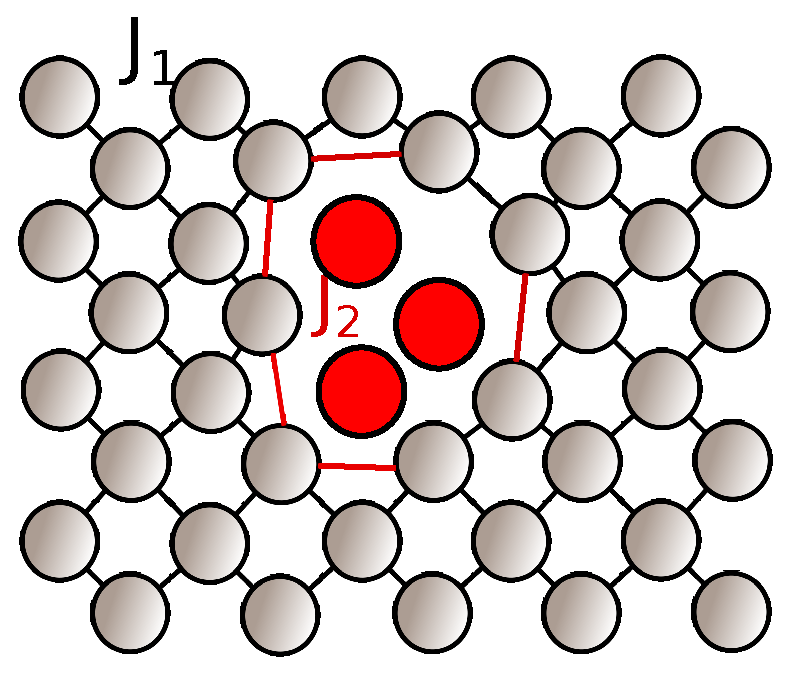
\includegraphics[height=4.5cm]{fig1a.eps}
\end{figure}
\begin{figure}[!t]
   \centering
   \hspace{0.8cm}
 {\scriptsize\textbf{(b)}}\\
   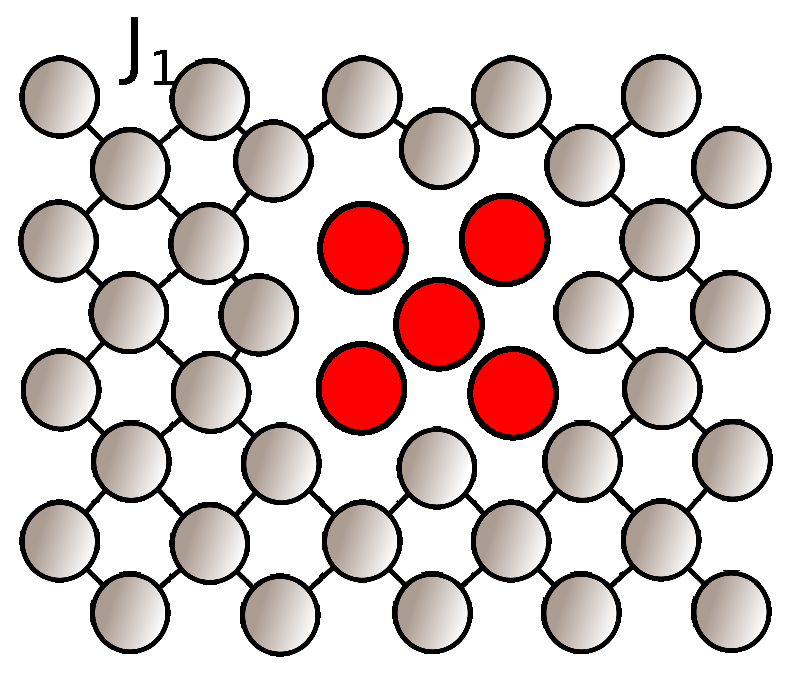
\includegraphics[height=4.5cm]{fig1b.eps}
\caption{(Color online) A lattice sketch of the induced superexchange interaction $J_2$ by the cluster dopant (disconnected
 circles) for $\Gamma=4$. In (a), tree dopant generates the NNN interaction $J_2$. In (b), a cluster of five dopants does not induce $J_2$.}
\label{fig0}
\end{figure}

%
The above Hamiltonian has been studied through Monte Carlo simulations. First, we prepare a diluted sample, i.e., to a given value of $p$, the algorithm builds an random matrix $\{\epsilon \}$, another algorithm sweeps the $\{\epsilon \}$ measuring the Al cluster size and using $\Gamma$ parameter to builds the $\{\zeta\}$ matrix. In figure \ref{fig0} a situation is represented for $\Gamma = 4 $, for cluster with lessr than $5$ impurities, Al atom induces superexchange interactions, otherwise it does not.
%

in this model, for every thermodynamic observable $Q$, we first calculate the thermal average $\langle Q_{\{\epsilon\}} \rangle$ for a given sample $\{\epsilon \}$ and the results for different samples are later average as $\left[ {\left\langle {Q_{\left\{ \epsilon \right\}} } \right\rangle }\right]_{{\text{av}}}$. In order to get the critical properties of the present model, for each sample of a given site-disorder configuration $p$, we used a hybrid Monte Carlo algorithm consisting of one single spin Metropolis algorithm \cite{newman1999monte}, and one cluster wolff algorithm \cite{wolff1989collective} . This hybrid Monte Carlo method~\cite{creutz, pawig} has been implemented, and has been shown to reduce correlations between successive configurations in the simulation. Close to the transition temperature we have also resorted to single histogram techniques to get the corresponding thermodynamic quantities. We have first computed the magnetization, magnetic susceptibility, and the Binder cumulant given, respectively, by
%

\begin{eqnarray}
m=\frac{1}{N}\sum_{i=1}^{N}S_{i},\\
\label{mag}
\chi_{} = N \frac{\langle m^{2}\rangle -\langle m \rangle
^{2}}{T},\\
u_{4}=1-\frac{\langle m^{4}\rangle}{3\langle m^{2}\rangle^2},
%\\
%\label{chi}
%u_{4}=1-\frac{\langle m_{x}^{4}\rangle}{3\langle m_{x}^{2}\rangle ^2},
\label{U1}
\end{eqnarray}
%
where $N=2L^3$ and $L$ is the linear size of the cubic lattice studied, $T$ is the temperature given in units of $J/k_B$, $k_B$ being the Boltzmann constant. We have also considered $J=1$, in such a way that $J_2$ is measured in units of $J$.
In addition, to reach the final results, for each dilution, temperature, and lattice size, the MC estimates $\langle Q_{\{\epsilon\}} \rangle$ of thermodynamic quantities, for a given random sample  $\{\epsilon\}$ of diluted sites were averaged over different disorder realizations as
%
\begin{equation}
\left[ {\left\langle {Q_{\left\{ \epsilon  \right\}} } \right\rangle } \right]_{{\text{av}}}  = \frac{1}
{{\# \left\{ \epsilon  \right\}}}\sum\limits_{\left\{ \epsilon  \right\}} {\left\langle {Q_{\left\{ \epsilon
\right\}} } \right\rangle } ,
\label{av}
\end{equation}
%
with $\#\{\epsilon\}$ the number of total realizations considered.
Now, regarding the simulational numbers, for every sample the runs comprised $ 3 \times 10^4$ MCS per spin for equilibration and  the measurements were made over $5 \times 10^5$ MCS. The lattice sizes raged from $L=10$, $20$, $30$ the values being chosen so that $p \times L^3$ gives an integer number. We have used in the present paper $50$ samples for all settings.


\section{Results}
\begin{figure}[htb]
\begin{center}
\includegraphics[width = 8.5cm]{fig1.eps}
\end{center}
\caption{(color online) Magnetic susceptibility as a function of the temperature for different samples. In this example, to $L=10$, $\Gamma=N=2000$, $\alpha=1.26$ and $\beta= 0.75$ . For a question of clarity, the Monte Carlo data have been omitted and only the lines are shown in this figure.}
\label{fig:1}
\end{figure}

In Fig. \ref{fig:1} it is shown the behavior of $\chi$ as a function of temperature for fifty samples, for concentration ranging from $p=0$ to $p=0.7$ with steps of $0.05$,  lattce size $L=10$, $\alpha=1.26$, $\beta= 0.75$, and $\Gamma = N = 2000$, i.e., all dopants induce superexchange interaction $J_2$. The temperature $T$ here is measured in units of the Boltzmann constant. These curves were obtained using the simple histogram technique. For each sample, the system presented a temperature and susceptibility value that was slightly different. We can observe that for values of $p =0 $ up to $p=0.5$ the susceptibility curves correspond to the same peak height. For $p >5$ the peaks increase and a greater variation between the samples. The peak of each of these samples is used to estimate the transition temperature $T_c(p)$.

\begin{figure}[htb]
\includegraphics[width = 7.4cm]{fig2.eps}
\caption{(Color online) Susceptibilidade vs critical temperature $T_c(p)$  for fifty samples and several values of $p$. With $\Gamma=2L^3$, $\alpha=1.26$ and $\beta= 0.75$ The simulational errors are smaller than the symbol sizes.}
\label{fig:2}
\end{figure}


In Fig. \ref{fig:2} it is shown the peak of each of the simulated samples. We can observe that the points become more dispersed as the concentration of dopants increases. Taking the mean of the $T_c$ of each sample and obtaining the temperature of the collection for a given configuration.



\begin{figure}[htb]
\includegraphics[width = 7.4cm]{fig3.eps}
\caption{(Color online) Phase diagram in the $T–q$ plane. Solid circles are the results of present model. Solid line is the previous fit using the Effective field theory  Ref \cite{Freitas2013}, star points are the experimental data. \ref{x,x,x} }
\label{fig:3}
\end{figure}

Fig. \ref{fig:3} exhibits the transition temperature $T_c(p)$ as a function of $p$ to the best result obtained with the adjustment of the $\alpha$, $\beta$ and $\Gamma$ parameters in comparison with the experimental results and  comparison with the results of Ref \cite{Freitas2013}.


\section{Conclusion}



\begin{thebibliography}{00}

\bibitem{Domb1983} R.B. Stinchcombe, in: C. Domb, J.L. Lebowitz (Eds.), Phase Transitions and Critical Phenomena, vol. 7, Academic Press, New York, 1983
\bibitem{Kubaschewski1982} Kubaschewski, O. (1982). Iron—Binary phase diagrams. Springer Science \& Business Media.
\bibitem{Menendez2009} Menéndez, Enric, et al. "Direct magnetic patterning due to the generation of ferromagnetism by selective ion irradiation of paramagnetic FeAl alloys." small 5.2 (2009): 229-234.
\bibitem{Bali2014} R. Bali, S. Wintz, F. Meutzner, R. Hbner, R. Boucher, A.A. nal, S. Valencia, A. Neudert, K. Potzger, J. Bauch, F. Kronast, S. Facsko, J. Lindner, J. Fassbender, Nano Lett. 14 (2014) 435.
\bibitem{Wolf11986} W. Wolf, Braz. J. Phys. 30(4), 794 (2000). 2G. A. P. Alcazar, J. A. Plascak, and E. G. Da Silva, Phys. Rev. B 34, 1940(1986).
\bibitem{Besnus1975} M. J. Besnus, A. Herr, and A. J. P. Meyer, J. Phys. F 5, 2138 (1975).
\bibitem{Dias2009} D. A. Dias, J. R. de Sousa, and J. A. Plascak, Phys. Lett. A 373, 3513 (2009).
\bibitem{Oubelkacem2010} A. Oubelkacem, I. Essaoudi, A. Ainane, F. Dujardin, J. Ricardo de Sousa, and M. Saber, Physica A 389, 3427 (2010)
\bibitem{Arrott1959} Arrott, Anthony, and Hiroshi Sato. "Transitions from Ferromagnetism to Antiferromagnetism in Iron-Aluminum Alloys. Experimental Results." Physical Review 114.6 (1959): 1420.
\bibitem{Shull1959} Shull, R. D., H. Okamoto, and P. A. Beck. "Transition from ferromagnetism to mictomagnetism in Fe—Al alloys." Solid State Communications 20.9 (1976): 863-868.
\bibitem{Boni1986} Böni, P., S. M. Shapiro, and K. Motoya. "Field induced modulated structure in the re-entrant spin glass Fe70· 4 Al29· 6 in applied magnetic fields." Solid state communications 60.11 (1986): 881-884.
\bibitem{Takahashi1996} Takahashi, S., X. G. Li, and A. Chiba. "Spin distribution in plastically deformed Fe-Al intermetallic compounds." Journal of Physics: Condensed Matter 8.50 (1996): 11243.
\bibitem{Perez1986} Alcázar, GA Pérez, J. A. Plascak, and E. Galvao da Silva. "Site-diluted Ising model for the magnetic properties of $Fe_{1− q}Al_q$, $0≤ q≤ 0.5$, alloys in the disordered phase." Physical Review B 34.3 (1986): 1940.
\bibitem{Sort2006} Sort, J.; Concustell, A.; Menéndez, E.; Suriñach, S.; Rao, K. V.; Deevi, S. C.; Baró, M. D.; Nogués, J. Adv. Mater. 2006, 18, 1717.
\bibitem{Trautvetter2011} Trautvetter, M.; Wiedwald, U.; Paul, H.; Minkow, A.; Ziemann, P. Appl. Phys. A: Mater. Sci. Process. 2011, 102 (3), 725.
\bibitem{Zamora2009} Zamora, L. E.; Pérez Alcázar, G. A.; Vélez, G. Y.; Betancur, J. D.; Marco, J. F.; Romero, J. J.; Martínez, A.; Palomares, F. J.; González, J. M. Phys. Rev. B 2009, 79, 094418.
\bibitem{Plascak2000} Plascak, J. A., Zamora, L. E., Alcazar, G. P. (2000). Ising model for disordered ferromagnetic Fe− Al alloys. Physical Review B, 61(5), 3188.
\bibitem{Koch2006} Koch, Carl C. Nanostructured materials: processing, properties and applications. William Andrew, 2006.
\bibitem{Mustalahti2015} Mustalahti, S., Myllyperkio, P., Malola, S., Lahtinen, T., Salorinne, K., Koivisto, J., Pettersson, M. (2015). Molecule-like Photodynamics of Au102 (p MBA) 44 Nanocluster. ACS nano, 9(3), 2328-2335.
\bibitem{newman1999monte} M. E. J. Newman, G. T. Barkema, GT,  \textit{Monte  Carlo methods in statistical physics}, {Oxford University Press, USA} \textbf{}  (1999).
\bibitem{wolff1989collective} U. Wolff, \textit{Phys. Rev. Lett.} \textbf{62} 361 (1989).
\bibitem{creutz} M. Creutz, \textit{Phys. Rev. D} \textbf{36}  515 (1987).
\bibitem{pawig}S. G. Pawig, K. Pinn, \textit{Int. J. Mod. Phys. C}  \textbf{9} 727  (1998).
\bibitem{Freitas2013} Freitas, A. S., de Albuquerque, D. F., Fittipaldi, I. P.,  Moreno, N. O. (2013). Study of the Fe-Al alloys in the Ising model for $S= 2$ spin by employing the effective field theory. Journal of Applied Physics, 113(9), 093903.
\end{thebibliography}
\end{document}
